\section{System Architecture and Design}

%[[ Explain the architecture layering, perhaps include some UML, and mention the
%technologies used.

%Remember a picture is worth a thousand words! ]]

\subsection{Architecture}
Initially, we planned to implement a traditional Model-View-Controller (MVC) architecture for our project, but due to React's component based nature, we adjusted our approach to better align with its framework. Instead of strictly adhering to MVC, we designed the architecture to leverage React's modular and reusable components. Each component in our project encapsulates specific functionality and is responsible for managing its own logic, user interactions, and html. These components return HTML like JS code, which is dynamically rendered and combined to form the user interface. The App.js file serves as the central hub of the application, acting somewhat like a controller in a traditional MVC setup. It orchestrates the application by importing and rendering the various components based on the user's interactions and the current application state. Moreover, the React-based approach blends the Model and View into individual components. For instance, GameTable.js manages the game logic (model) while simultaneously rendering the game table (view) to the user. While this architecture differs from a strict MVC implementation, it retains the core benefits of modularity and scalability.

\subsection{Technologies}
Since we developed a web-based version of the card game "War," we decided to use modern web technologies to create a responsive and scalable application. Our front end consisted of common web development technologies: HTML, CSS, and JavaScript. HTML provided the basic structure of the web page, while CSS allowed us to style the page according to the theme specified by Cosmic Radiance. JavaScript handled the game logic on the client side. We used React.js as our front-end framework to facilitate updating the game state without refreshing the page. React also helped us create reusable components, such as the cards themselves.
Our back end handled the game logic, player data, and real-time communication. We used Node.js to manage game logic outside of the browser, which enabled us to handle requests like determining winners.
To store user data, game history, and player stats, we needed persistent storage. We chose Firebase for this purpose due to its ease of use with real-time updates. Firebase provided a flexible schema compared to SQL databases, which require defined relationships among tables. It also included built-in authentication, supporting Google and Facebook sign-ins as well as traditional email and password login. Overall, Firebase met our needs for real-time updates, scalability, security, and rapid development.




\subsection{Coding Standards}
Our database naming scheme consisted of singular, lowercase names for collections (user, leaderboard). Each attribute within documents used camelCase (userName, gameStats, gameID). Variables and functions in JavaScript were also written in camelCase.

We formatted our code using two spaces for indentation. Brackets were placed on the same line for functions and other control statements. Inline comments were used only to explain complex logic, while multi-line comments were used to describe functions and classes. Additionally, all functions were properly documented with a multi-line comment describing their purpose, parameters, and return value.

Our testing standards followed a test-driven development approach. We ensured proper functionality by requiring all code commits to pass necessary code tests before merging. These tests accounted for correctness, edge cases, and performance.

\subsection{UML Diagram}
\begin{figure}
    \centering
    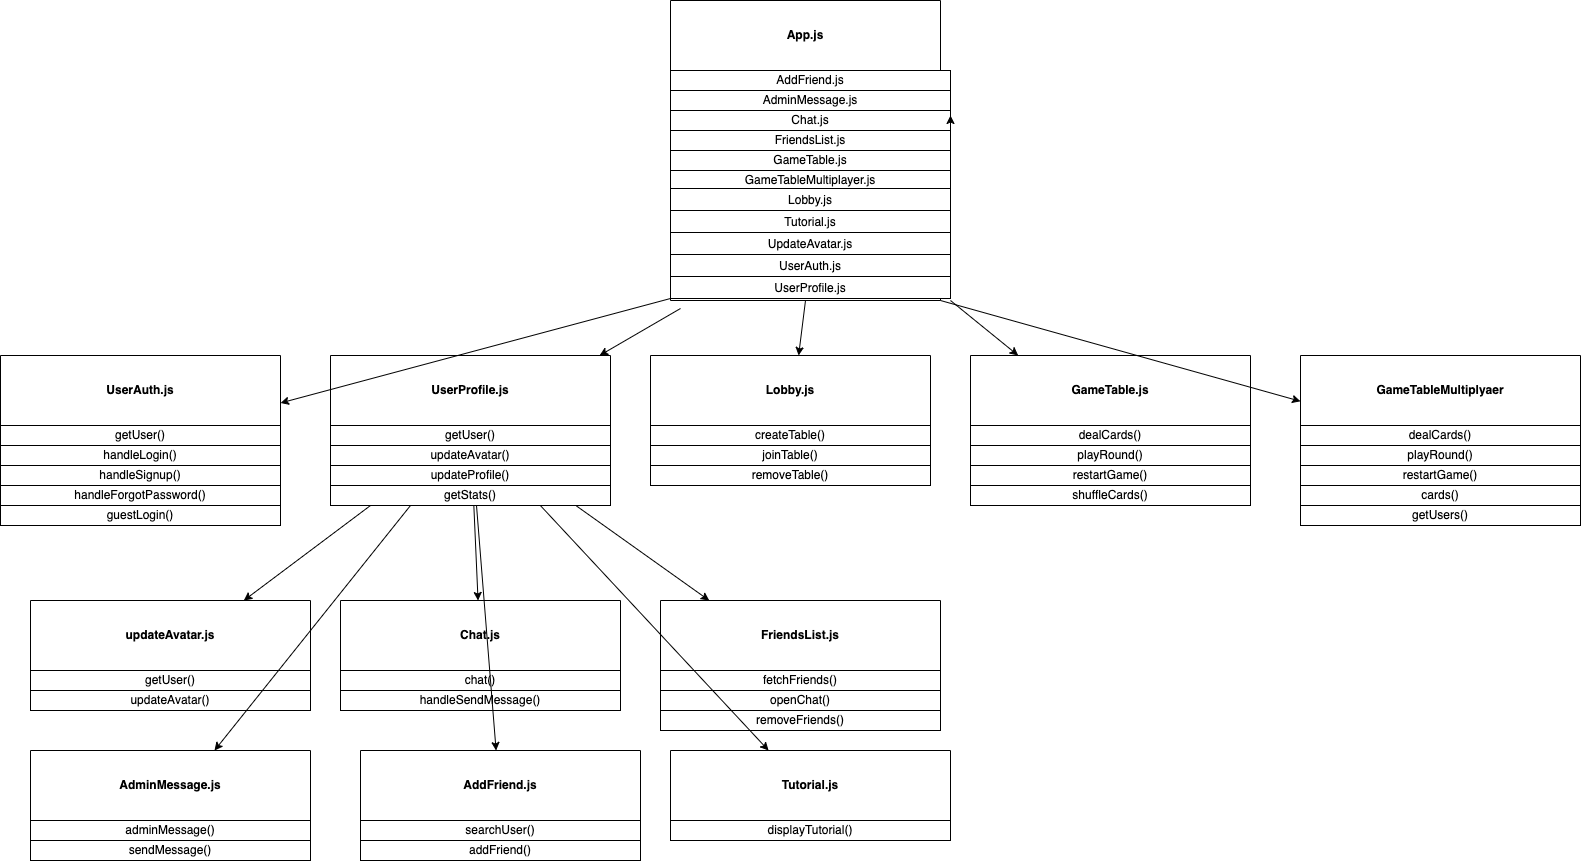
\includegraphics[width=1\linewidth]{figures/finalUML.png}
    \caption{UML diagram outlining the war card game for Cosmic Radiance}
    \label{fig:enter-label}
\end{figure}

\begin{figure}
    \centering
    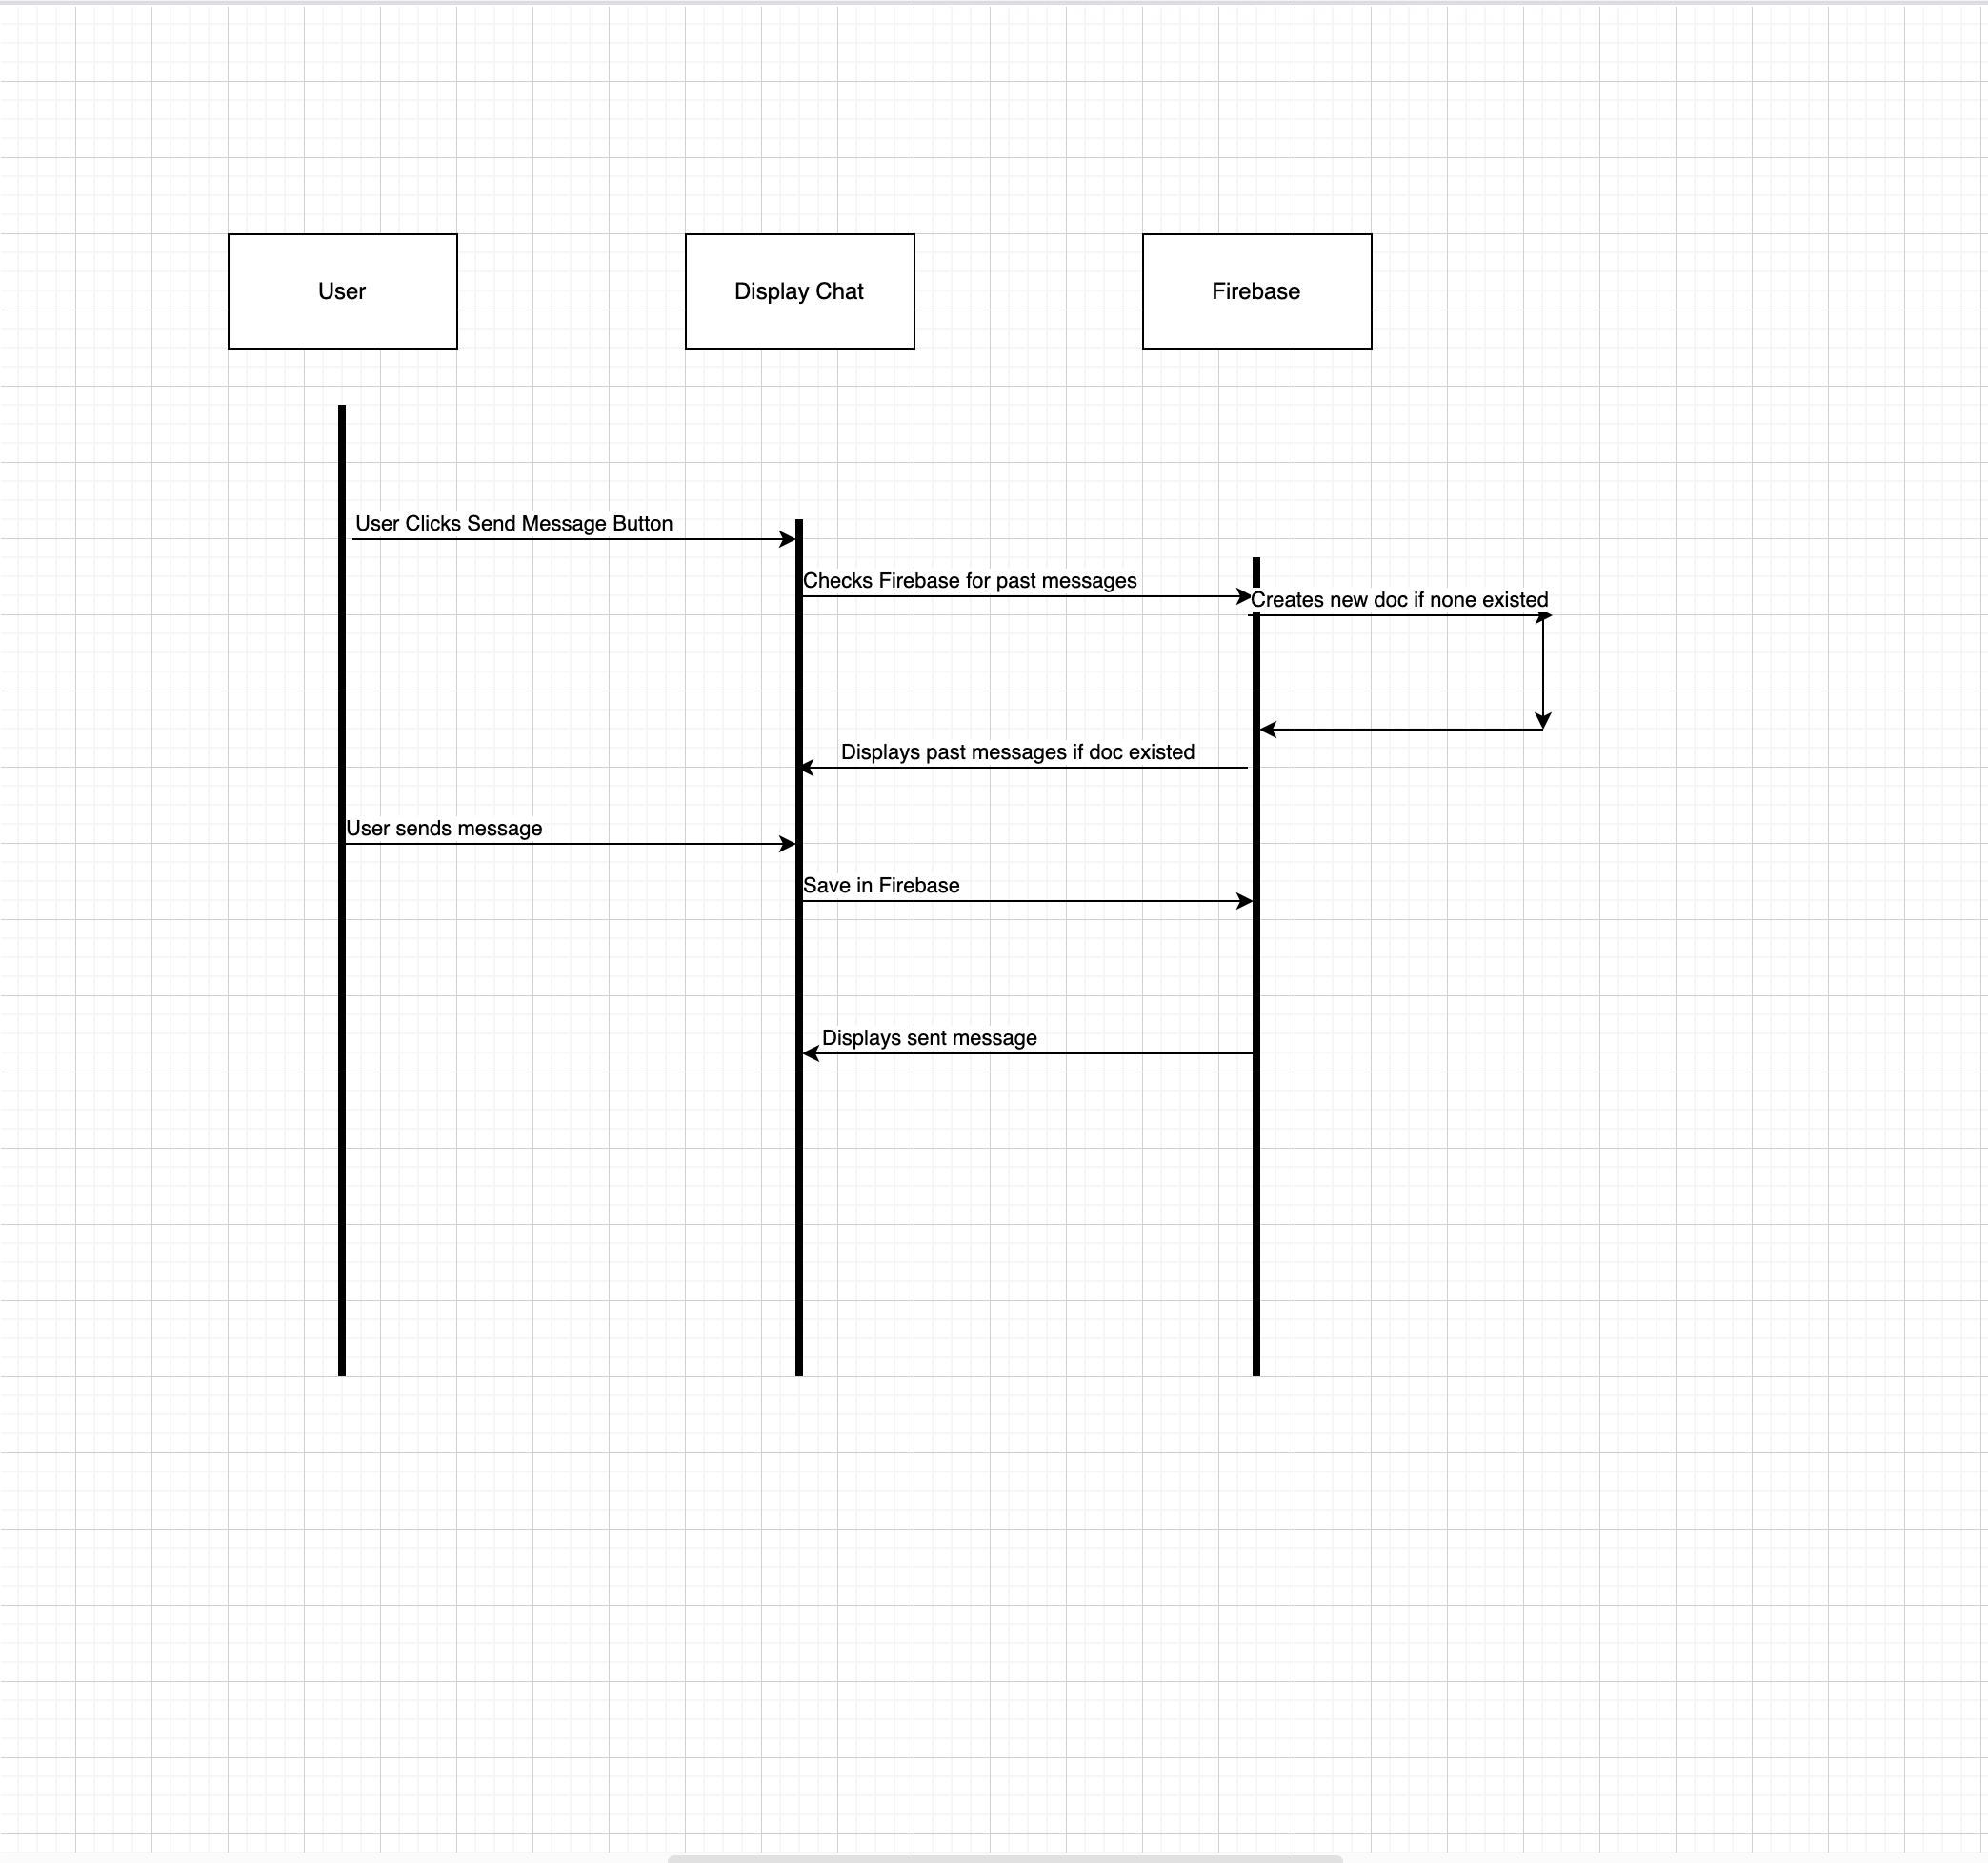
\includegraphics[width=1\linewidth]{documentation/figures/Sequence UML .png}
    \caption{UML Sequence diagram for chat of War}
    \label{fig:enter-label}
\end{figure}

This UML diagram illustrates the component-based architecture of the War card game application. It highlights the relationships between classes, such as App.js, which orchestrates key components like UserAuth.js, GameTable.js, and Lobby.js. The diagram also shows the methods and interactions within each class.




